\documentclass[a4paper,oneside]{memoir}
% Divide report into subfiles
\usepackage{subfiles}

\usepackage[english]{babel}
\usepackage[margin=1cm]{caption}
\usepackage[T1]{fontenc}
\usepackage[utf8]{inputenc}
\usepackage{wallpaper}
\usepackage{palatino}
\usepackage{hyperref}
\usepackage{csquotes}
\usepackage{fvextra}
\usepackage{xpatch}
\usepackage{amsmath}

% tikz drawing
\usepackage{tikz}
\usetikzlibrary{shapes,arrows,matrix,chains,positioning,decorations.pathreplacing,arrows}

% Listings
\usepackage{listings}
\lstset{
  basicstyle=\ttfamily,
  mathescape
}

% Proofs
\usepackage{bussproofs}

% Floats and figures
\usepackage{float}
\usepackage{wrapfig}
\restylefloat{figure}
\usepackage{caption}
\DeclareCaptionLabelFormat{cont}{#1~#2\alph{ContinuedFloat}}
\captionsetup[ContinuedFloat]{labelformat=cont}

%linespacing
\usepackage{setspace}
\renewcommand{\baselinestretch}{1.5}

% Grammar
\usepackage{fancyvrb}

% Internal references
\usepackage{cleveref}

% Bibliography
\usepackage[style=authoryear]{biblatex}
\addbibresource{bib.bib}
\bibliography{bib}

% Promote sections and subsections
\setheadfoot{\onelineskip}{2\onelineskip}
\setheaderspaces{*}{1mm}{*}

% Glossary
\usepackage[numberedsection=nameref]{glossaries}
\renewcommand{\glossarypreamble}{\label{glos}}
\makeglossaries
\newglossaryentry{agent} {
  name = agent,
  description = {An agent is a system that can act based on previous knowledge,
		 and that can \textit{learn} to adapt its actions.
	         Used interchangeably with \textit{system}}
}
\newglossaryentry{ai} {
    name = artificial intelligence,
    description = {Artificial intelligence (AI) covers the broad discipline in computer science
that is concerned with replicating intelligent behaviour in computational systems. The exact
definition is controversial for historical reasons \autocite{Nilsson2009}}
}
\newglossaryentry{ANN} {
  name = artificial neural network,
  description = {
    Artificial neural networks is a broad term for connected units with 
    weighted edges.
    Each unit is roughly modelled over the biological neuron, in the way 
    that they can receive a number of inputs (dendrites) 
    but only provide a single output (axon).
    They also typicall use sigmoidal activation functions to calculate the 
    unit responses.
    This broad definition covers both third and second generation neural
    networks, and is generally avoided througout the thesis to avoid 
    ambiguity}
}
\newglossaryentry{API} {
  name = API,
  first = {application programming interface (API)},
  description = {A number of interaction-points for a piece of code,
		 such as a library or framework, that are available for
		 other programmers to communicate with. APIs are typically
		 documented as lists of their modular components along
		 with their purpose and usage}
}
\newglossaryentry{ARM} {
  name = {ARM},
  description = {A family of reduced instruction set computing (RISC) for 
                 processing units that are widespread in smaller and mobile
		 devices.}
}
\newglossaryentry{backend} {
  name = backend,
  description = {...}
}
\newglossaryentry{BrainScaleS} {
  name = BrainScaleS,
  description = {...}
}
\newglossaryentry{computation} {
   name = computation,
   description = {Computation refers to any process (in any
substrate) that can deduce new information based on old information. In
this is manifested as computing instructions}
}
\newglossaryentry{CSA} {
  name = {connection-set algebra},
  description = {...}
}
\newglossaryentry{DARPA} {
  name = {DARPA},
  description = {The Defense Advanced Research Projects Agency is an agency
                 in the Department of Defense in the United States, who
		 have funded---and are funding---a number of emerging information
		 and military technologies.}
}
\newglossaryentry{DL} {
  name = {DL},
  first = {deep learning (DL)},
  description = {...}
}
\newglossaryentry{DNN} {
  name = {deep neural network},
  description = {Deep neural networks...}
}
\newglossaryentry{DSL} {
  name = {DSL},
  first = {domain specific language (DSL)},
  description = {A DSL is a language used to model concepts from a certain
    domain. DSLs are usually simpler than more general programming languages in
    that they contain fewer concepts and less complex syntax}
}
\newglossaryentry{FPGA} {
  name = {FPGA},
  description = {A field-programmable gate array (FPGA) is a programmable
		 integrated circuit, that can achieve high-speed computing
		 by wiring physical blocks together to perform high-speed
		 computations.}
}
\newglossaryentry{Futhark} {
   name = {Futhark},
   description = {A programming language geared towards performance in parallel environment such as
   graphics processors (GPUs). Futhark is a purely functional array language and is
   developed by HIPERFIT research center under the Department of Computer Science at the
   University of Copenhagen (DIKU)}
}
\newglossaryentry{HBP} {
  name = HBP,
  first = {Human Brain Project (HBP)},
  description = {...}
}
\newglossaryentry{NEST} {
  name = NEST,
  description = {...}
}
\newglossaryentry{NN} {
  name = {neural network},
  description = {A neural network refers to a circuit of neurons, artificial or biological.}
}
\newglossaryentry{ncc} {
   name = {NCC},
   description = {Neural patterns or condition that is minimally sufficient for a conscious
thought to occur. See \autocite{atkinson2000, Hohwy2009}}
}
\newglossaryentry{ml} {
  name = machine learning,
  description = {Machine learning is a sub-field within \gls{ai} that is concerned
    with developing systems that ``progressively improves their performance on a
    certain task'' \autocite{wiki:ml}}
}
\newglossaryentry{meme} {
name = meme,
description = {\textit{Meme} is a shortened form of the ancient Greek \textit{mimeme} meaning
`imitated thing' and was coined by Richard Dawkins. A meme refers to a idea or a
\textit{way of behaving} that can be \enquote{copied, transmitted, remembered, taught, shunned,
brandished, ridiculed, parodied, censored, hallowed} \autocite{dennett2017}}
}
\newglossaryentry{Myelin} {
  name = Myelin,
  description = {...}
}
\newglossaryentry{OpenCL} {
   name = {OpenCL},
   description = {An open standard for cross-platform parallel programming, which
   allows software to be executed on CPUs, GPUs or other processors or hardware accelerators. See \url{
   https://www.khronos.org/opencl/}}
}
\newglossaryentry{Python} {
  name = Python,
  description = {...}
}
\newglossaryentry{RAM} {
  name = RAM,
  description = {Random-access memory (RAM) is a temporary storage device
	         that allows read and write access to arbitrary locations
		 without significant delays compared to spinning disks.
		 Typically used as a cache for instructions and memory
		 from long-term storage.}
}
\newglossaryentry{REF} {
  name = REF,
  first = {Reorganisation of Elementary Functions (REF)},
  description = {A theory and model for rehabilitation in patients
  with brain lesions, developed by \cite{Mogensen2011}.
  An extension in the form of the REFGEN model was developed by
  \textcite{Mogensen2017} to account for broader aspects of
  neurocognitive organisation.}
}
\newglossaryentry{SNN} {
  name = SNN,
  first = {spiking neural network (SNN)},
  description = {A broad term for second or third generation neural
                 networks whose nodes communicates via timed pulses or
		 \textit{spikes}}
}
\newglossaryentry{vonNeumann} {
  name = {von Neumann architecture},
  description = {A computer architecture for universal computing machines that
                 relies on a processing unit, a control unit and memory for
		 storing data and instructions. Invented by John von Neumann in
		 1945.}
}

\makeglossaries

% TOC
\maxsecnumdepth{subsection}

% \raggedbottom

% Chapter settings
\chapterstyle{ger}

% Change memoir chapter margins
\usepackage{titlesec}
\titleformat{\chapter} % command
  [display] % shape
  {\normalfont\huge\bfseries} % format
  {\chaptertitlename\ \thechapter} % label
  {5pt} % Separator
  {
    % \rule{\textwidth}{1pt}
    % \vspace{1ex}
    % \centering
  } % Before code
  [
    \vspace{-0.5ex}
    \rule{\textwidth}{0.3pt}
  ] % after code

% \titlespacing*{\chapter}{10pt}{10pt}{10pt}

%%  Setup fancy style quotation
%%  ==================================================================
%\usepackage{tikz}
%\usepackage{framed}

%\newcommand*\quotefont{\fontfamily{fxl}} % selects Libertine for quote font

% Make commands for the quotes
%\newcommand*{\openquote}{\tikz[remember picture,overlay,xshift=-15pt,yshift=-10pt]
%     \node (OQ) {\quotefont\fontsize{60}{60}\selectfont``};\kern0pt}
%\newcommand*{\closequote}{\tikz[remember picture,overlay,xshift=15pt,yshift=5pt]
%     \node (CQ) {\quotefont\fontsize{60}{60}\selectfont''};}

% select a colour for the shading
%\definecolor{shadecolor}{rgb}{1,1,1}

% wrap everything in its own environment
%\newenvironment{shadequote}%
%{\begin{snugshade}\begin{quote}\openquote}
%{\hfill\closequote\end{quote}\end{snugshade}}

%%  Begin document
%%  ==================================================================
\begin{document}

%%  Begin title page
%%  ==================================================================
    \thispagestyle{empty}
    \ULCornerWallPaper{1}{ku-coverpage/nat-farve.pdf}
    \ULCornerWallPaper{1}{ku-coverpage/diku-en.pdf}
    \begin{adjustwidth}{-3cm}{-1.5cm}
    %\vspace*{-1cm}
    %\textbf{\Huge Free topic} \\
    \vspace*{2.5cm}
    \textbf{\Huge Modelling learning systems} \\
    \vspace*{.8cm}
    {\huge Modelling learning in spiking neural networks}\\
    \begin{tabbing}
    % adjust the hspace below for the longest author name
    Jens Egholm Pedersen \hspace{1cm} \= \texttt{<xtp778@alumni.ku.dk>} \\
    \\[11cm]

    \textbf{\Large Supervisor} \\
    Martin Elsman \hspace{1cm} \texttt{<mael@di.ku.dk>}
    \end{tabbing}
    \end{adjustwidth}

    \newpage

    \ClearWallPaper
%%  ==================================================================
%%  End title page

\renewcommand\cftchapteraftersnumb{\normalfont}
\renewcommand\cftbeforechapterskip{5pt plus 1pt}

\frontmatter
\setcounter{tocdepth}{2}
\tableofcontents*
\newpage

\mainmatter
\chapter{Introduction} \label{sec:intro}
  \subfile{chapters/introduction}

\chapter{Theory}
  \subfile{chapters/theory}

\chapter{Neural network modelling in Volr} \label{sec:volr}
  \subfile{chapters/volr}

\chapter{Neural network architecture} \label{sec:model}
  \subfile{chapters/model}

\chapter{Experimental setup} \label{sec:experiment}
  \subfile{chapters/experiment}

\chapter{Data collection}
  \section{Futhark}
  \section{NEST}
  \section{BrainScaleS}

\chapter{Analysis}
  \section{Experiment results}
  \subsection{Futhark}
  \subsection{Nest}
  \subsection{BrainScaleS}
  \section{Comparison of learning}
  \section{Adaptability and robustness} % How is this useful for the REF model?

\chapter{Discussion}
  \section{Validity}
  \section{REF similarity}
  \section{Future work}

\chapter{Conclusion}

\printbibliography

\appendix
\chapter{Volr} \label{appendix:volr}
  \documentclass{report.tex}{subfiles}
\begin{document}
Before diving into the actual experiment built to test the hypothesis, this
chapter discusses and describes the method employed to model spiking
and artificial \gls{NN}s.

Both types of network are architecturally similar, and both are conceived from
the same physiological principles \autocite{dayan2001, russel2007, Nilsson2009, schmidhuber2014}.
The implementations, however, vary greatly.

To ensure internal and external validity in and between the two network types,
it is desirable that the models are as closely related from a theoretical and
practical perspective as possible.
Additionally, to test the hypothesis, it is required that both the artificial
and spiking models can be simulated on regular machine architecture, while
the spiking model requires a neuromorphic hardware platform.

An optimal approach would be to find a tool that leverages the similarities
of the network types, while integrating with the diverse simulated or emulated
targets.
That is, an abstract model of neural networks that can translate into
heterogeneous back-ends, while retaining a high degree of inter-model validity.

A number of general frameworks for artificial neural networks
exist\footnote{
  Among others, see \autocite{ONNX2018}, \autocite{PyTorch2018}, \autocite{TensorFlow2018},
  \autocite{Keras2018} and DyNet \autocite{Neubig2017}.
}, but none of them extend to the spiking domain.
Conversely a number of choices exist for neuromorphic modelling\footnote{
  %TODO: Find sources on internal IBM/Intel stuff
}, but they exclusively evaluate to neuromorphic or spiking neural network
backends \autocite{Jordan2018}.

A domain-specific language (DSL) called Volr was recently presented to
construct reproducible \gls{NN} experiments
\autocite{Pedersen2018:volr}.
The DSL allows the modelling of sufficiently complicated models for
the purpose of this thesis, while providing a set of tools that permits the
model be sent and evaluated on both \gls{ANN} and \gls{SNN} targets.

Some work was required to fully support learning mechanisms on
neuromorphic hardware, and the DSL, as well as the tooling around it, has been
extended for the purpose of this thesis (see appendix \ref{appendix:volr})
The following section describes the grammar and anatomy of Volr in detail.

\section{Volr}
Volr is a declarative DSL designed to model \gls{NN} that seeks a
trade-off between complete, but verbose, descriptions of small
networks and more general designs of large and complex networks.
By separating the network topologies from the detailed physiological properties
of each neuron or neuron population, the language aims to allow simple
experiments with few, concise declarations, as well as larger and more
complicated experiments while retaining readability.

Figure \ref{fig:volr-expr} shows the BNF form of expressions, values and types
in Volr, while figure \ref{fig:volr-rules} lists evaluation rules to apply
when evaluating the expressions.
Finally the \ref{fig:volr-examples} shows an example network that solves
a rudimentary maze task.
% Expressions, evaluation rules and examples
% Expression figure
\begin{figure}
  \begin{tabular}[t]{l l}
    expressions 
    & \texttt{$e$ ::= $n$} \\
    & \begin{minipage}{0.6\textwidth}
      \begin{Verbatim}[mathescape,commandchars=\\\{\}]
    | \textbf{stim} $n$
    | \textbf{pop} $n\ m$
    | \textbf{tar} $n$
    | $e \otimes e$
    | \textbf{let} $x = e$ \textbf{in} $e'$
      \end{Verbatim} 
    \end{minipage} \\
    & \\ % Empty space
    values
    & \texttt{$v$ ::= $n$} \\
    & \\ % Empty space

    types
    & \texttt{$\tau$ ::= \textbf{group} $n\ m$ | \textbf{stimt} $n$ | \textbf{int} }
  \end{tabular}

  \caption{Expressions, values and types of the Volr language.}
  \label{fig:volr-expr}
\end{figure}

\begin{figure}
\begin{prooftree}
  \AxiomC{}
  \RightLabel{\hskip10pt($e1$)}
  \UnaryInfC{$\Gamma \vdash n : \mathbf{int}$}
\end{prooftree}
\begin{prooftree}
  \AxiomC{}
  \RightLabel{\hskip10pt($e2$)}
  \UnaryInfC{$\Gamma \vdash \mathbf{stim}\ n : \mathbf{net}\ 1\ n$}
\end{prooftree}
\begin{prooftree}
  \AxiomC{}
  \RightLabel{\hskip10pt($e3$)}
  \UnaryInfC{$\Gamma \vdash \mathbf{pop}\ n : \mathbf{net}\ 1\ n$}
\end{prooftree}
\begin{prooftree}
  \AxiomC{$\Gamma (x) = \tau$}
  \RightLabel{\hskip10pt($e4$)}
  \UnaryInfC{$\Gamma \vdash x : \tau$}
\end{prooftree}
\begin{prooftree}
  \AxiomC{$\Gamma \vdash e_1 : \mathbf{net}\ l\ m$}
  \AxiomC{$\Gamma \vdash e_2 : \mathbf{net}\ n\ q$}
  \AxiomC{$\Gamma \vdash w : \mathbf{float}$}
  \RightLabel{\hskip10pt($e5$)}
  \TrinaryInfC{$\Gamma \vdash \otimes\ e_1\ e_2\ w : \mathbf{net}\ l\ q$}
\end{prooftree}
\begin{prooftree}
  \AxiomC{$\Gamma \vdash e_1 : \mathbf{net}\ l\ m$}
  \AxiomC{$\Gamma \vdash e_2 : \mathbf{net}\ m\ n$}
  \AxiomC{$\Gamma \vdash w : \mathbf{float}$}
  \RightLabel{\hskip10pt($e6$)}
  \TrinaryInfC{$\Gamma \vdash \ominus\ e_1\ e_2\ w : \mathbf{net}\ l\ n$}
\end{prooftree}
\begin{prooftree}
  \AxiomC{$\Gamma \vdash e : \tau$}
  \AxiomC{$\Gamma [v : \tau] \vdash e' : \tau$}
  \RightLabel{\hskip10pt($e7$)}
  \BinaryInfC{$\Gamma \vdash \mathbf{let}\ x = e\ in\ e' : \tau$}
\end{prooftree}

  \caption{Evaluation rules in Volr.}
  \label{fig:volr-rules}
\end{figure}



\begin{figure}
  \ContinuedFloat*
  \begin{tabular}[t]{l c}
    \begin{minipage}{0.4\textwidth}
      \begin{Verbatim}[mathescape,commandchars=\\\{\}]
\textbf{dense} 2 2
      \end{Verbatim}
    \end{minipage} & \begin{minipage}{0.4\textwidth}
      \includegraphics[width=\textwidth]{chapters/volr/example2.pdf}
    \end{minipage}

  \end{tabular}
  \caption{A network with a stimulus containing two channels.
    The stimulus is fully connected to a population with an excitatory
    weight of 1. Each circular node represents a single neuron.}
  \label{fig:volr-example1}
\end{figure}

\begin{figure}
  \ContinuedFloat
  \begin{tabular}[t]{l c}
    \begin{minipage}{0.4\textwidth}
      \begin{Verbatim}[mathescape,commandchars=\\\{\}]
\textbf{let} s$_1$ = \textbf{dense} 1 1 \textbf{in}
\textbf{let} s$_2$ = $\neg$ \textbf{dense} 1 1 \textbf{in}
(s$_1$ $\ominus$ s$_2$) $\obar$ \textbf{dense} 2 1
      \end{Verbatim}
    \end{minipage} & \begin{minipage}{0.6\textwidth}
      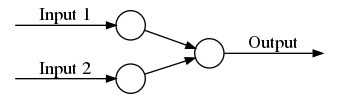
\includegraphics[width=\textwidth]{chapters/volr/example1.pdf}
    \end{minipage}
  \end{tabular}
  \caption{An illustration of a simple binary network, whose two 
	   parallel layers share the middle population of size 2.}
\end{figure}

\begin{figure}
  \ContinuedFloat
  \begin{tabular}[t]{l c}
    \begin{minipage}[b]{0.4\textwidth}
      \begin{Verbatim}[mathescape,commandchars=\\\{\}]
      \textbf{dense} 100 50
        $\obar$ \textbf{dense} 50 10
      \end{Verbatim}
    \end{minipage} & \begin{minipage}{0.5\textwidth}
      \includegraphics[width=\textwidth]{chapters/volr/example3.pdf}
    \end{minipage}
  \end{tabular}
  \caption{A larger network that can process the MNIST dataset
    as 10x10 pixel images. 
    The nodes are populations of neurons,
    where the input corresponds to the pixel size ($10\cdot10=100$) 
    and the output to the possible classes (0 - 9).
    Input and output are implicit.}
\end{figure}

\begin{figure}
  \begin{tabular}[t]{l c}
    \begin{minipage}{0.45\textwidth}
      \begin{Verbatim}[mathescape,commandchars=\\\{\}]
\textbf{let} s = \textbf{dense} 2 2 \textbf{in}
\textbf{let} l$_1$ = \textbf{dense} 2 4 \textbf{in}
\textbf{let} l$_2$ = \textbf{dense} 2 4 \textbf{in}
\textbf{let} o = \textbf{dense} 8 1 \textbf{in} 
  s $\obar$ (l$_1$ $\ominus$ l$_2$) $\obar$ o
      \end{Verbatim}
    \end{minipage} & \begin{minipage}{0.5\textwidth}
       \includegraphics[width=\textwidth]{chapters/volr/example4.pdf}
    \end{minipage}
  \end{tabular}
   \caption{An example where a two-dimensional input is split into
     two nodes and later merged into a node of a single neuron.}
  \label{fig:volr-examples}
\end{figure}



\newpage\null\thispagestyle{empty}\newpage
\newpage\null\thispagestyle{empty}\newpage
\pagebreak
Figure \ref{fig:volr-bnf} shows the constituent parts of an experiment.
Four sub-com\-po\-nents are required:
  A number of stimuli, neural populations, responses and experiment targets.

\subsubsection{Block grammar} \label{sec:volr-block}
The sub-components are constructed using the same declarative \textit{block}
structure shown in figure \ref{fig:volr-ebnf-block}.
The block defines its \textit{type} (\texttt{stimulus}, \texttt{population},
\texttt{response} or \texttt{target}), an optional \textit{name} and lastly
some block content.

The content varies for the different block types, but is restricted to contain
a number of either key-value pairs (\texttt{field}s) or relations to other
blocks (\texttt{connection}s).
Fields are interpreted by the respective targets (see section
\ref{sec:volr-targets}) and connections are only allowed for
\texttt{population}s and \texttt{responses}.

\subsubsection{Connection-set algebra grammar} \label{sec:volr-csa}
Connections between blocks are implemented as a subset of the \gls{CSA}
introduced in section \ref{sec:CSA} \autocite{Djurfeldt2012}.
Most notably, the notion of \textit{blocks} and \textit{geometric distance} have
been omitted\footnote{Neither blocks nor distances are required for the
  experiment in the thesis. It is, however, a necessary element to conduct
  further experiments, since biological \gls{SNN} are highly influenced by
  spatial arrangements \autocite{dayan2001}.
}.

The grammar is presented in figure \ref{fig:volr-ebnf-csa}, and aims to provide
a flexible way to describe complex connectivity patterns in text.
The present grammar can be viewed as a basic algebraic tool for set operations.
Describing full connectivity between two populations, such that all neurons
in the first population is connected with all neurons in the second population,
can simply be expressed as `\texttt{all}'.
Connecting one neuron to one other neuron between two populations are described
as `\texttt{one}', while random connectivity are described with a probability
of, say 0.5: `\texttt{random 0.5}'\footnote{
  This expresses a Bernouilli trial with the given probability
  \autocite{Djurfeldt2012}.
}
As a final example, every neuron in a population connected to every neuron in
that same population, with the exception of identical neurons, can be described
as `\texttt{all - self}'.
%
% \begin{figure}
%   \begin{center}
%     \begin{minipage}{0.8\linewidth}
%       \begin{grammar}
%         <connection> ::= 'from' , <block-name> , { <csa-expr> } ;
%
%         <csa-expr> ::= <csa-term> | <csa-expr> , <csa-operator> , <csa-expr> ;
%
%         <csa-term> ::= 'all' | 'one' | 'self' | 'random' , <number> ;
%
%         <csa-operator> ::= '+' | '-' | '*' ;
%       \end{grammar}
%     \end{minipage}
%   \end{center}
%   \caption{BNF of the connection grammar, describing relations between
%     blocks through \gls{CSA}.}
%   \label{fig:volr-bnf-csa}
% \end{figure}

\subsubsection{Experiment stimuli}
The stimuli describes the ``input'' of the model.
Such input is defined either as an array of elements directly in the DSL
or as a reference to a file.

\subsubsection{Experiment populations}
The populations describe the topology of the neural network itself.
As with the stimuli, the populations are built around a block structure that
contains a number of sub-expressions.

The \texttt{connection} defines the source stimulus for the population,
i.e. the population \textit{from} which action-potentials will be forwarded.
A population can receive stimulus from more than one source.
The connections are modelled as per the \gls{CSA} described in section
\ref{sec:volr-csa}.

% TODO: Describe and invent archetypes... or not?

\subsubsection{Experiment responses}
The responses are the ``output'' of the model to be recorded, and can be
considered as the outcome of the network for training purposes.
The response block only contains an optional specification of a location for
the experiment output data.

\subsubsection{Experiment targets}
The final element in a Volr experiment is its targets.
A target describe a destination environments on which to run the experiment.
These are described in detail in section \ref{sec:volr-targets}, and are
referenced in the grammar as simple strings.

\subsection{Volr semantics}
In practice a network is built by describing a graph.
The nodes in the graph consist of \texttt{populations} of neurons and the edges
are connection-set matrices to other populations \autocite{Djurfeldt2012}.
% TODO: Describe CSA
\texttt{Populations} can consist of any positive number of neurons and is
required to have at least one connection.
Connections can be recursive, resulting in a potentially cyclic graph.
Both the connections and the \texttt{populations} can be annotated with features
such as connection weight and neuron parameters (see \nameref{appendix:volr}).
The parameters are treated differently depending on the experiment target (see
sections \ref{sec:volr-NEST} and \ref{sec:volr-BrainScaleS}).


\section{Neural network simulation targets in Volr} \label{sec:volr-targets}

% TODO :Write how fields are interpreted
% TODO: Write how input is interpreted

Volr exploits the structural similarities between \gls{ANN} and \gls{SNN} to
translate the model to both spiking and artificial network platforms (back-ends).

In the remainder of the chapter the three emulation back-ends, shown in figure
\ref{fig:volr}, are described:
a machine learning target for \gls{ANN}s and a neuron simulation target, as well
as a neuromorphic hardware target, for \gls{SNN}s.

\begin{figure}
  \centering
  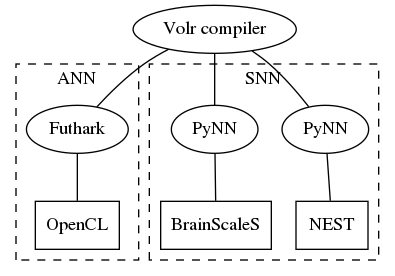
\includegraphics[width=0.6\textwidth]{images/volr-architecture.png}
  \caption{The translation from the Volr DSL to \gls{ANN} simulations in OpenCL via
    \gls{Futhark} and to \gls{SNN} simulations on \gls{NEST} and \gls{BrainScaleS}
    via the \gls{Myelin} middleware.
  }
  \label{fig:volr}
\end{figure}

\subsection{Translation to Futhark} \label{sec:volr-futhark}
Futhark is a functional data-parallel programming language \autocite{Henriksen2017}.
It offers a number of compilation targets such as \gls{OpenCL}, which is
particularly interesting for this thesis because of its capacity for hardware
acceleration.

The practical translation from the Volr model to Futhark is built on recurrent
\gls{ANN} with stochastic gradient descent backpropagation
\autocite{russel2007, schmidhuber2014}.
Each neuron population is considered as a single layer, whose connections are
determined by a connection matrix.

% Deal with recurrent connections
% Describe how this relates to layers

... To be continued ...

\subsection{Spiking neural network simulations via PyNN} \label{sec:volr-pynn}
The Python neural network simulation interface PyNN is designed as a
"simulator-independent language for building neuronal network models"
\autocite{PyNN2018}.
It aims to reduce the problem of diverse, and occasionally unique, descriptions
of neural network experiments for different simulation back-ends \autocite{Davison2009}.
PyNN has been adapted by a number of simulators, including the NEST simulation
platform and the neuromorphic BrainScaleS wafer system
\autocite{Davison2009, Helias2012, Schmitt2017}.

There are still simulator-dependent configurations that seems unlikely to be
adopted into PyNN in the immediate future\footnote{
  Particularly hardware mapping configurations are hard to abstract in a general
  interface.
}.
For that reason Volr provides simulation-specific PyNN scripts that can
interpret the model in the context of each simulation target.
A middleware, dubbed \gls{Myelin}, was invented to translate the \gls{NN} model
into a static intermediate representation in JSON.
The JSON standard was chosen for the task because of its concise syntax while
still retaining human readability.

The advantage of the static experiment representation being, that the experiment
easily a) transports to the target PyNN scripts without losing any information,
and b) duplexes between several experiment; the same experiment setup is
trivial to setup on multiple targets at once.

The correct execution of the experiments relies on the PyNN scripts to exploit
the simulator to represent the Volr model as accurately as possible.
Fortunately PyNN is designed to cover exactly such a use case, so properties
related to the \gls{NN} models itself (such as network topology and population
attributes) were faithfully reproduced across the simulators.
However, the simulators deviate in a number of ways that are relevant to
mention.
The following two sections explains the steps necessary to achieve accurate
experiment environments in \gls{NEST} and \gls{BrainScaleS}.

\subsubsection{Translation to PyNN} \label{sec:volr-translation}

\subsubsection{Translation to NEST} \label{sec:volr-NEST}
... To be continued ...
\subsubsection{Translation to BrainScaleS} \label{sec:volr-BrainScaleS}
... To be continued ...
\end{document}

\end{document}
